\documentclass[tikz]{standalone}
\usepackage[utf8]{inputenc}
\usetikzlibrary{calc,intersections}

\definecolor{DarkBlue}{rgb}{0.0,0.0,0.6}

\begin{document}

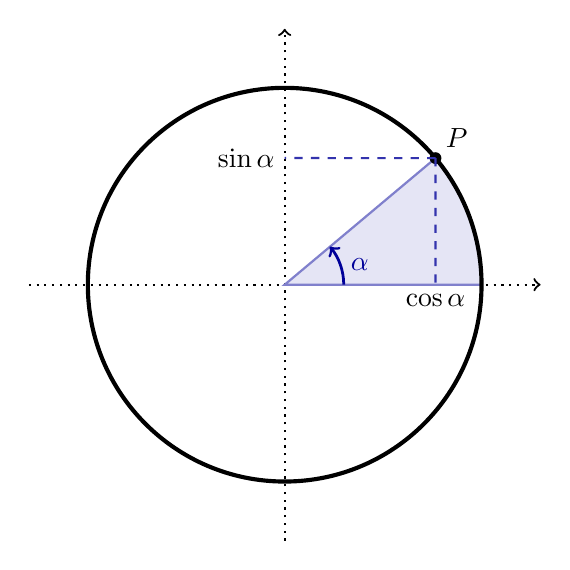
\begin{tikzpicture}[thick,scale=2.5]
\def\ptsize{.03}
\draw[->,dotted] (-1.3, 0) -- (1.3,0);
\draw[->,dotted] (0,-1.3) -- (0,1.3);
\coordinate (inf) at (1,0);
\draw[DarkBlue!50,fill=DarkBlue!10] (0,0) -- (inf) arc (0:40:1) -- cycle;
\path[draw,name path=circ,line width=1.5pt] (0,0) circle (1);
\coordinate[label=above right:$P$] (P) at (40:1);
\fill (P) circle (\ptsize);
\draw[DarkBlue,line width=1pt,->] (.3,0) arc (0:40:.3) node[midway, right] {$\alpha$};
\path let \p1 = (P) in node[below] (cos) at (\x1,0) {$\cos\alpha$}
                       node[left] (sin) at (0,\y1) {$\sin\alpha$};
\draw[DarkBlue!80,dashed] (P) -- (cos);
\draw[DarkBlue!80,dashed] (P) -- (sin);
\end{tikzpicture}

\end{document}